\chapter{04 Forelesnings Notater}
\section{Compton-Spredning}
\subsubsection{Sentrale kunnskaper}
\begin{itemize}
    \item Beskrive de fysiske modellene
    \item Vite at fotoner har bevegelsesmengde
    \item fotoner kolliderer med frie elektroner, eller med tunge atomer 
    \item Brakk-diffraksjon
    \item Utlede formel for compton-bølgelengde $λ_c$
    \item Beskrive hvordan fotonet tilordnes både partikkel- og bølge-egenskaper. 
    \item Formler for energi og bevegelsesmengde 
\end{itemize}

\subsubsection*{Oblig 1 denne uken}
\[
\frac{\mathrm{d}^{2}f(x)}{\mathrm{d}x^{2}} = ϵ f(x)
\]
\subsubsection*{Repetisjon}
\begin{itemize}
    \item Elektromegnetiske bøgleer består av energipakker (fotoner)
    \item 
    Et foton:
    \item Har en bølgelengde $λ = \frac{c}{ν}$ og energi $E = hν$
    \item Oppfører seg også som en partikkel
\end{itemize}
  
  
\subsection{Oppsett}
\begin{figure}[h!]
  \centering
  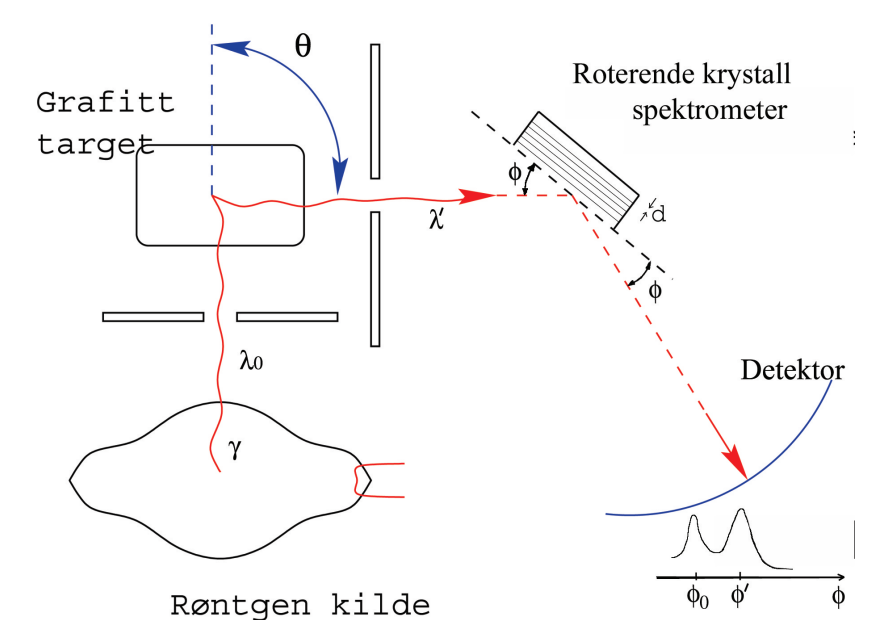
\includegraphics[scale = .4]{Figures/Compton oppsett.png}
  \caption{Oppsett av forsøk for Compton spredning}
  \label{fig: Compton oppsett}
\end{figure}

Vi sender Röntgenstråling med energi $E_0 = hν = h c / λ_0$ en hvis bølgelengde, på et mål laget av grafitt. Det kolliderer med elektronene i materialet, og skyter ut et nytt foton med ca. samme bølgelengde og energi. Dette fotonet kolliderer i krystall spektrometeret. Krystallen har flere lag som fotonet kan kollidere med. Flere fotoner kan da ha konstruktiv interferens med hverandre gitt ved $nλ = 2d \sin ϕ$, der d er tykkelsen på krystallen, $n$ er et heltall og at $ϕ$ er innfallsvinkelen. Noen ganger kommer det et fotonet med større bølgelengde og dermed mindre energi. Denne spredningen av fotonene sin energi som sett nederst til høyre i figur \ref{fig: Compton oppsett} kalles Compton spredning. En fant også ut at hvis en endrer vinkelen $θ$ fra 90 grader til 45 grader skaper en større spredning som sett i \ref{fig: Compton resultater}. 

\subsection{Forklaring}

\begin{figure}[h!]
  \centering
  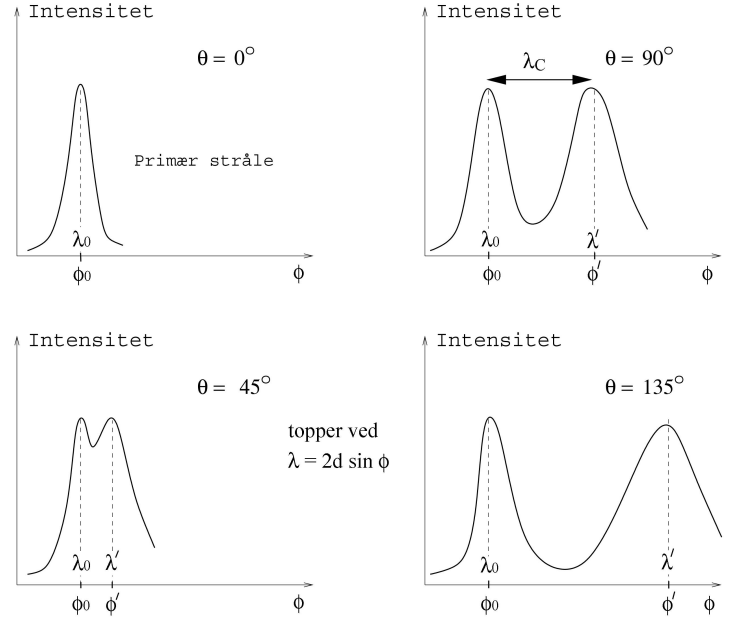
\includegraphics[scale = .5]{Figures/Compton resultater.png}
  \caption{Resultat ved compton eksperiment}
  \label{fig: Compton resultater}
\end{figure}

Einstein forstod at hvis energien til fotonet var redusert måtte det også bety en reduksjon i bevegelsesmengde HVIS en er på fotonet som en partikkel. Han mente fotoner har følgende egenskaper: 
\begin{enumerate}
    \item $E = høn = h c / λ$
    \item $E = mc^2 \frac{1}{\sqrt{1 - v^{2} / c^{2}}} ⇒ v = c, \quad m = 0$
    \item $E = \sqrt{p^{2} c^{2} +(mc^{2})^{2}} ⇒ p = E /c = hν / c = h /λ$
\end{enumerate}
Einstein tenkte da at energi og bevegelsesmengde må være bevart. Hvis en tenker at elektronene står stille vil da fotonet ha bevegelsesmengde $p_{γ_{x}}$ og $p_{γ_{y}}$ og elektronet bevegelsesmengde $p_{e} = 0$ 




\subsubsection*{Før}
Foton: 
\begin{itemize}
    \item $E_{γ} = h c / λ_0$
    \item $p_{γ_{x}} = h / λ_0$
    \item $p_{γ_{y}} = 0$  
\end{itemize}

Elektron
\begin{itemize}
    \item $E_{e} = m_e c^{2}$
    \item $p_e = 0$
\end{itemize}

\subsubsection*{Etter}
Foton: 
\begin{itemize}
    \item $E_{γ}' = h c / λ'$
    \item $p_{γ_{x}}' = h / λ' \cos θ$
    \item $p_{γ_{x}}' = -h / λ' \sin θ$
\end{itemize}

Elektron: 
\begin{itemize}
    \item $E_{e}' = \sqrt{p^{2} c^{2} + m_e^{2}c^{4}}$
    \item $p_{e_{x}}' = p_e' \cos ζ$
    \item $p_{e_{y}}' = p_e' \sin ζ$
\end{itemize}
  

\begin{figure}[h!]
  \centering
  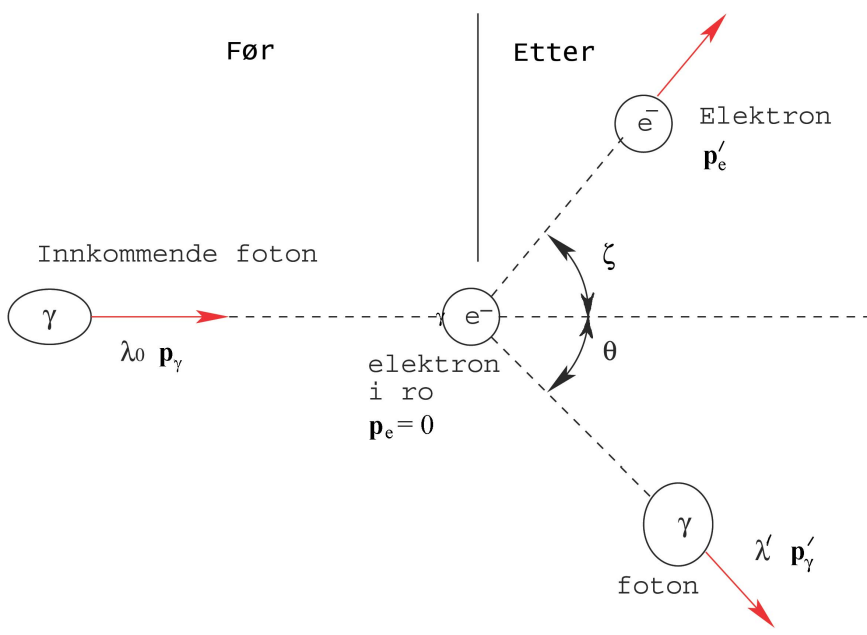
\includegraphics[scale = .5]{Figures/kollisjon elektron og foton.png}
  \caption{Kollisjon mellom elektron og foton}
  \label{fig: kollisjon elektron og foton}
\end{figure}


\[
\frac{hc}{λ_0} + m_e c^{2} = \sqrt{p^{2} c^{2} + m_e^{2}c^{4}} + \frac{hc}{λ'}
\]
\[
\left( \frac{hc}{λ_0} - \frac{hc}{λ'} + m_e c^{2}  \right)^{2} = p^{2} c^{2} + m_e^{2}c^{4}
\]
\[
\frac{h^{2}c^{2}}{λ_0^{2}} + \frac{h^{2}c^{2}}{λ'^{2}} - 2 \frac{h^{2}c^{2}}{λ_0 λ'} + \cancel{m_e^{2} c^{4}} + 2 m_e c^{2} \left( \frac{hc}{λ_0} - \frac{hc}{λ'} \right) = p^{2} c^{2} + \cancel{m_e^{2}c^{4}}
\]

\[
Δ λ = ( λ' - λ_0) = \frac{h}{m_e c} (1 - \cos θ)
\]
Som en konsekvens av ligningen over ser vi at maksimal spredning kommer av en vinkel $θ = 180^{\text{o}}$. 

Compton's Bølgelengde defineres som:
\[
λc = \frac{hc}{m_e c^{2}} = 0.00243 \text{ nm}
\]
\[
Δ λ_{\text{max}} = 2 λ_c = 0.0048 \text{ nm}
\]
Som vi ser i figur \ref{fig: Compton resultater} ser vi at uavhengig av spredning vil vi få samme $λ_0$ som tilsvarer en $ϕ_0$. Dette er fordi at fotonet også kan treffe store atomer som beveger seg ekstremt lite. \colorbox{red}{Hvilken av toppene tilsvarer hvilken type kollisjon ?}